\documentclass[10pt,twocolumn]{article}
\usepackage[letterpaper,top=0.75in,bottom=1in,left=0.65in,right=0.65in,columnsep=0.25in]{geometry}
\usepackage{times,graphicx,booktabs,amsmath,amssymb,cite,url,caption,float}
\captionsetup{font=footnotesize,labelfont=bf,labelsep=period}
\renewcommand{\thesection}{\Roman{section}}
\renewcommand{\thesubsection}{\Alph{subsection}.}
\setlength{\parindent}{1em}\setlength{\parskip}{0pt}
\makeatletter
\renewcommand{\section}{\@startsection{section}{1}{0pt}{8pt}{4pt}{\centering\normalfont\small\scshape}}
\renewcommand{\subsection}{\@startsection{subsection}{2}{0pt}{5pt}{2pt}{\normalfont\small\itshape}}
\newcommand{\tb}[1]{\textbf{#1}}
\makeatother
\newcommand{\ind}{\mathbb{1}}
\begin{document}
\twocolumn[{
\begin{center}
{\LARGE\bfseries Identifying Regime Changes in Indian Financial Markets\\ using Change Point Detection}\\[4pt]
{\large Detection, Event Validation and Out-of-Sample Forecasting Value}\vspace{8pt}\\
\begin{tabular}{cc}
Aditya Ranka & Parth Bagal\\
\small School of Humanities and Basic Sciences & \small School of Humanities and Basic Sciences\\
\small Manipal Institute of Technology & \small Manipal Institute of Technology
\end{tabular}\vspace{8pt}
\end{center}
\begin{quote}\small\itshape
\tb{Abstract}---We study change point detection (CPD) as a non-parametric tool for identifying regime changes in the NIFTY~50 (2007--2025) and ask whether regime information has forecasting value. Offline PELT with a Gaussian cost on daily returns yields 16 breakpoints; 56\% of nine documented stress events fall within $\pm$20 trading days of a break, against 14\% for randomly placed breaks. This measures \emph{localisation} of shifts after the fact, not prediction. For prediction we run a strictly out-of-sample, weekly walk-forward experiment (637 forecasts, 2013--2025) with ridge regression for next-21-day realised volatility and L2 logistic regression for a $>$5\% drawdown flag. Trailing and EWMA volatility give an out-of-sample $R^2$ of 0.33 over an expanding-mean benchmark. Adding the CPD or HMM regime features does \emph{not} improve it (relative $R^2$ change: CPD $-$2.2\%, $p=0.62$; HMM $-$1.2\%, $p=0.28$), while India VIX does (+16.6\%, $p=0.006$). No model discriminates the drawdown flag (AUC 0.49--0.56; every bootstrap interval for the gain over the baseline contains zero). In a regime-switching allocation, all rules cut maximum drawdown ($-$38\% to about $-$26\%) but only the HMM rule improved the Sharpe ratio, and a static 60/40 NIFTY/gold mix beat all of them. Regimes describe volatility well but add no measurable forecasting information beyond standard volatility inputs.
\par\smallskip\tb{Keywords}---Change Point Detection, Regime Change, Hidden Markov Model, Volatility Forecasting, Walk-forward Validation, Ridge Regression, Logistic Regression, Portfolio Allocation
\end{quote}
\vspace{4pt}
}]

\section{Introduction}
Financial markets alternate between calm and stressed periods. Classical portfolio and risk models assume stationary returns, which regime changes violate: the NIFTY~50 daily log-returns used here have an excess kurtosis of 15.2 and visible volatility clustering (Fig.~\ref{fig:eda}). Hidden Markov Models (HMMs) are the conventional regime tool \cite{hamilton,angtim} but fix the number of states and the emission distribution in advance. Change point detection locates the times at which the statistical properties of a series shift, without a generative model \cite{truong}. We ask four questions: (i) does offline CPD localise known stress shifts in Indian equity data; (ii) how does it compare with an HMM; (iii) can regime information \emph{forecast} future volatility or drawdowns once strict out-of-sample discipline is imposed; and (iv) does it help a simple allocation rule?

A point of framing matters for (iii). A change point is, by construction, a change that has \emph{already happened}: detecting it needs post-shift data, so it cannot anticipate the news that caused it. What can be forecastable is what follows a detected shift, because volatility is persistent. We therefore test regime features as predictors of \emph{future} volatility and drawdown, against strong baselines, rather than as predictors of the shift itself.

\section{Related Work}
Killick, Fearnhead and Eckley introduced PELT, an exact offline segmentation algorithm with expected linear cost under a penalised-cost formulation \cite{killick}. Truong, Oudre and Vayatis survey CPD methods and provide the \textit{ruptures} library used here \cite{truong}. Ang and Timmermann review regime switching in asset returns and its implications for allocation and risk \cite{angtim}; Markov-switching models originate with Hamilton \cite{hamilton}. Volatility persistence is the basis of EWMA/RiskMetrics forecasts \cite{rm}. Forecast comparison uses the Diebold--Mariano test \cite{dm} with a Newey--West long-run variance \cite{nw}; dependent-data resampling uses the moving block bootstrap \cite{kunsch}. Bayesian online CPD \cite{adams} is left for future work.

\section{Data and Preprocessing}
Daily adjusted closes were downloaded from Yahoo Finance: NIFTY~50 (Sep.\ 2007--Dec.\ 2025, 4{,}485 returns), India VIX (from Mar.\ 2008), and two NSE-traded ETFs used as allocation assets: Gold BeES (gold) and Liquid BeES (cash proxy), both from Jan.\ 2009. Let $P_t$ be the NIFTY close and $r_t=\ln(P_t/P_{t-1})$ the log-return. Allocation returns are clipped at $\pm$30\% to guard against bad ticks. The VIX series is forward-filled over non-trading gaps. All data are daily; no intraday data are used.

\begin{figure}[t]\centering
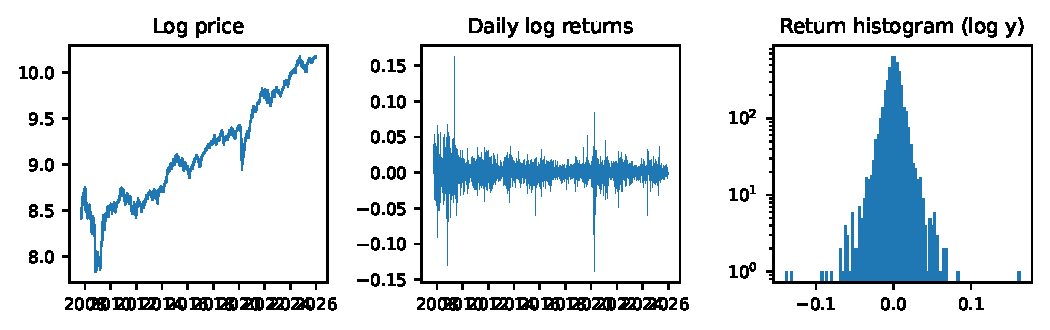
\includegraphics[width=\columnwidth]{../figures/eda.pdf}
\caption{NIFTY~50 log-price, daily log-returns and return histogram (log scale).}\label{fig:eda}
\end{figure}

\section{Regime Detection Methods}
\subsection{Change point detection (PELT)}
Given a series $y_{1:n}$, PELT \cite{killick} solves $\min_{K,\tau}\sum_{i=0}^{K}c\big(y_{\tau_i+1:\tau_{i+1}}\big)+\beta K$, where $c$ is a segment cost and $\beta$ a penalty. We use (a) the Gaussian cost with free mean and variance (\textit{ruptures} model ``normal'') on standardised returns, and (b) a least-squares (``l2'') cost on the standardised log of the 21-day realised volatility. Binary segmentation \cite{truong} with the same cost is used for comparison. Constraints: minimum segment length 20 trading days; candidate breakpoints on a 5-day grid (\textit{jump}=5). The penalty is the main tuning choice: for a sample of length $n$ we set $\beta=3\ln n$ (a BIC-style rule for three parameters per segment), i.e.\ 25.2 on the full sample ($n=4{,}485$) and 19.9 on the 750-day windows used in the walk-forward experiments. Fig.~\ref{fig:pen} shows the breakpoint count falling from 84 to 3 as $\beta$ goes from 5 to 160. $\beta$ was fixed a priori and not tuned on any outcome.

\begin{figure}[t]\centering
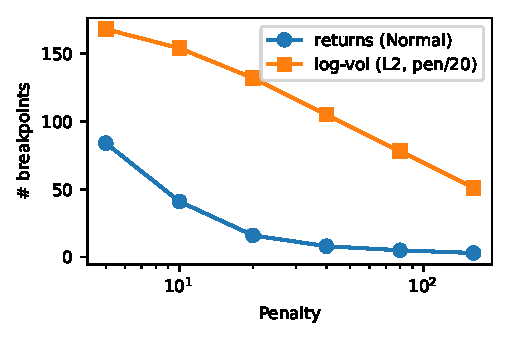
\includegraphics[width=0.8\columnwidth]{../figures/penalty_sweep.pdf}
\caption{Breakpoints versus penalty $\beta$.}\label{fig:pen}
\end{figure}

\subsection{Regime labelling}
A segment is labelled \emph{stress} if its annualised return volatility exceeds $1.3\times$ the median 21-day realised volatility (full sample: median 14.3\%, threshold 18.7\%). In walk-forward use, the median is taken over the trailing window only.

\subsection{HMM benchmark}
A two-state Gaussian HMM with full (here scalar) covariance is fitted by EM (Baum--Welch, up to 200 iterations) on standardised returns. We use 5 random initialisations on the full sample (seeds 0--4) and 3 in the walk-forward experiments (seeds 0--2), keeping the fit with the highest log-likelihood on the fitting window. The state with the larger fitted variance is called \emph{stress}. For a window $x_{1:T}$, the feature we use is the posterior probability $P(S_T=\text{stress}\mid x_{1:T})$ of the \emph{last} observation; at the final point the smoothed posterior equals the filtered one, so it uses no data after $T$. Full-sample regime \emph{changes} are the dates at which the Viterbi-decoded state switches.

\section{Event Validation: Localisation, Not Prediction}
We use nine documented stress events (Table~\ref{tab:ev}). For a margin $m$ in trading days, \emph{recall} is the share of events with a detected break within $m$ days (either side), and \emph{precision} the share of breaks within $m$ days of an event. Both depend on the number of breaks, so we also report expected values for $k$ uniformly random breaks (2{,}000 draws). \emph{Interpretation:} offline PELT uses the whole sample, so a break near an event shows that the estimator \emph{places} a detected shift close to the known event; it does not show that the shift could have been detected before or at the time of the news. The symmetric $\pm m$ window also treats early and late hits alike. Forecasting value is therefore tested separately (Section~\ref{sec:fc}).

\begin{table}[t]\centering\caption{Events used for validation (dates are approximate: the first major index move; to be verified against sources).}\label{tab:ev}
\footnotesize\begin{tabular}{@{}ll@{}}\toprule
Event & Date\\\midrule
Lehman / global financial crisis & 2008-09-15\\
US downgrade / euro-crisis sell-off & 2011-08-08\\
Taper tantrum & 2013-06-03\\
China devaluation sell-off & 2015-08-24\\
Demonetisation & 2016-11-08\\
IL\&FS credit crisis & 2018-09-21\\
COVID-19 crash & 2020-03-12\\
Russia--Ukraine / Fed tightening & 2022-02-24\\
2024 general-election result & 2024-06-04\\\bottomrule
\end{tabular}\end{table}

\section{Forecasting Experiment: ML Setup}\label{sec:fc}
\subsection{Problem statement}
Two supervised tasks are defined at each forecast date $d$, using only information strictly before $d$.
\emph{Task V (regression):} predict the log realised volatility over the next $H=21$ trading days.
\emph{Task D (classification):} predict whether the next 21 trading days contain a cumulative drawdown worse than 5\%.
The question is whether CPD- and HMM-based regime features improve on standard volatility predictors, \emph{incrementally}.

\subsection{Samples and information set}
Forecast dates $d_i$ are the first trading day of each ISO calendar week, from the first date with 750 prior returns (2010-10-11) to the last date with 21 subsequent returns (2025-12-01): $N=791$ samples. Let $\mathcal{I}_d$ be all data dated before $d$ (up to the close of the previous trading day). Every feature is a function of $\mathcal{I}_d$ only (Table~\ref{tab:feat}); returns from day $d$ onward are used only to build the targets.

\subsection{Targets}
Write $r_{d+k}$ for the return on the $k$-th trading day after $d$ ($k=0$ is day $d$ itself). Then
\begin{align}
y^{V}_d&=\ln\!\Big(\sqrt{252}\;\hat s\big(r_{d},\dots,r_{d+H-1}\big)\Big),\\
y^{D}_d&=\ind\!\Big[\min_{0\le k\le H-1}\Big(e^{\sum_{j=0}^{k}r_{d+j}}-1\Big)\le-0.05\Big],
\end{align}
where $\hat s$ is the sample standard deviation (denominator $H-1$). The base rate of $y^D$ is 16.6\% over all samples and 13.5\% over the out-of-sample set (86 positives of 637). Let $t^{\mathrm{end}}_d$ be the date of the last return in the target window.

\begin{table*}[t]\centering\caption{Features. All are computed from data before the forecast date $d$. $W=750$ is the window length; $\sigma_{21}$ and $\sigma_{\mathrm{ewma}}$ are annualised.}\label{tab:feat}
\footnotesize\begin{tabular}{@{}llp{4.6in}@{}}\toprule
Symbol & Name & Definition\\\midrule
$x_1=\ln\sigma_{21}$ & trailing vol & $\sigma_{21}=\sqrt{252}\;\hat s(r_{d-21},\dots,r_{d-1})$ (the 21 returns before $d$)\\
$x_2=\ln\sigma_{\mathrm{ewma}}$ & EWMA vol & $s_t^2=\lambda s_{t-1}^2+(1-\lambda)r_t^2$, $\lambda=0.94$ (RiskMetrics), $s^2$ initialised at $r_{\mathrm{first}}^2$; $\sigma_{\mathrm{ewma}}=\sqrt{252\,s^2_{d-1}}$\\
$x_3=\ln \mathrm{VIX}$ & India VIX & last India VIX close before $d$\\
$x_4=\ln(\hat\sigma_{\mathrm{seg}}/m_W)$ & CPD segment vol ratio & On the last $W$ returns, standardise with window mean/std; run PELT (Gaussian cost, $\beta=3\ln W$, min size 20, jump 5); $\hat\sigma_{\mathrm{seg}}=\sqrt{252}\,\hat s$ of the \emph{last} segment (raw returns); $m_W$ = median of $\sigma_{21}$ over the same window\\
$x_5=\ind[\hat\sigma_{\mathrm{seg}}>1.3\,m_W]$ & CPD stress flag & binary version of $x_4$\\
$x_6=P(S_T{=}\text{stress})$ & HMM stress prob. & 2-state Gaussian HMM on the same standardised window (Section~IV-C); posterior probability of the stress state at the last observation\\\bottomrule
\end{tabular}\end{table*}

\subsection{Feature sets (incremental design)}
To isolate the \emph{marginal} value of regime information, models differ only in which features they use:
\textbf{F0} $\{x_1,x_2\}$ (baseline); \textbf{F1} F0$+\{x_4,x_5\}$ (CPD); \textbf{F2} F0$+\{x_6\}$ (HMM); \textbf{F3} F0$+\{x_3\}$ (VIX); \textbf{F4} F0$+\{x_3,x_4,x_5,x_6\}$ (all); \textbf{VIX-only} $\{x_3\}$; \textbf{CPD+HMM-only} $\{x_4,x_5,x_6\}$. Additional non-fitted references for Task V: the \emph{expanding mean} of $y^V$ and the \emph{naive} forecast $\hat y^V=x_1$.

\subsection{Models}
\textbf{Task V: ridge regression.} For training pairs $(\mathbf z_j,y_j)$ with standardised features $\mathbf z_j$,
\begin{equation}
(\hat b,\hat{\mathbf w})=\arg\min_{b,\mathbf w}\sum_j\big(y_j-b-\mathbf w^{\top}\mathbf z_j\big)^2+\alpha\|\mathbf w\|_2^2,\quad\alpha=1,
\end{equation}
with an unpenalised intercept; the forecast is $\hat y=\hat b+\hat{\mathbf w}^{\top}\mathbf z$.
\textbf{Task D: L2 logistic regression.} With $\tilde y_j\in\{-1,+1\}$,
\begin{equation}
\min_{b,\mathbf w}\;\tfrac12\|\mathbf w\|_2^2+C\sum_j\ln\!\big(1+e^{-\tilde y_j(b+\mathbf w^{\top}\mathbf z_j)}\big),\quad C=1,
\end{equation}
giving $\hat p=\sigma(\hat b+\hat{\mathbf w}^{\top}\mathbf z)$, solved by L-BFGS (at most 1000 iterations). If a training set contains a single class, the training base rate is used. Both models use \textit{scikit-learn} defaults except as stated. \emph{Hyperparameters ($\alpha$, $C$, $\lambda$, $W$, $\beta$, $H$, the 5\% threshold) were fixed in advance and never tuned}, so there is no validation set and no hyperparameter-selection leakage; the price is that the models are not optimised. Standardisation is $\mathbf z=(\mathbf x-\boldsymbol\mu)/\boldsymbol\sigma$, with $\boldsymbol\mu,\boldsymbol\sigma$ computed on the training set only.

\subsection{Walk-forward protocol and leakage control}
For each sample $i$ in time order:
\begin{enumerate}\itemsep0pt
\item Training set $\mathcal{S}_i=\{j:\ t^{\mathrm{end}}_j<d_i\}$. This \emph{embargo} excludes any earlier sample whose 21-day target window had not finished before $d_i$, so no training target uses information unavailable at $d_i$ (about the last four weekly samples are dropped).
\item If $|\mathcal{S}_i|<150$ (about three years), make no forecast. The first out-of-sample forecast is 2013-09-23; there are 637 forecasts to 2025-12-01.
\item Fit the scaler and each model on $\mathcal{S}_i$ only; predict sample $i$; store the prediction.
\item Move to the next week and refit from scratch (expanding window).
\end{enumerate}
The regime features are recomputed at each $d_i$ from the trailing window only (PELT and the HMM are refit on the last 750 returns), so they contain no look-ahead. The HMM is not a trained component of the downstream model; only its output $x_6$ is a feature. Consecutive 21-day targets overlap by about 80\%, so forecast errors are serially correlated; the tests below account for this.

\subsection{Evaluation}
Let $e_{m,i}=y_i-\hat y_{m,i}$ over the $T=637$ out-of-sample forecasts.
\textbf{Regression:} RMSE, MAE, and the out-of-sample $R^2$
\begin{equation}
R^2_{\mathrm{OOS}}(m\mid \mathrm{ref})=1-\frac{\sum_i e_{m,i}^2}{\sum_i e_{\mathrm{ref},i}^2},
\end{equation}
reported against two references: the expanding mean ($R^2_{\mathrm{mean}}$) and the baseline F0 ($R^2_{\mathrm{F0}}$; positive means the model beats F0).
\textbf{Significance:} Diebold--Mariano test \cite{dm} on the squared-error loss differential $\delta_i=e_{\mathrm{F0},i}^2-e_{m,i}^2$: $\mathrm{DM}=\bar\delta/\sqrt{\hat V/T}$, with $\hat V=\hat\gamma_0+2\sum_{\ell=1}^{L}\big(1-\tfrac{\ell}{L+1}\big)\hat\gamma_\ell$ (Bartlett/Newey--West weights \cite{nw}), $L=H-1=20$; two-sided $p$-value from the standard normal; no small-sample correction.
\textbf{Classification:} ROC AUC, Brier score $\frac1T\sum_i(\hat p_i-y_i)^2$ and log loss, against a base-rate benchmark (training-set frequency). The AUC gain over F0 is given with a 95\% percentile interval from a moving block bootstrap \cite{kunsch}: blocks of 26 consecutive samples, 2{,}000 resamples (seed 0), resamples with a single class discarded.
\textbf{Descriptive checks:} out-of-sample mean next-21-day volatility and drawdown frequency conditional on each regime signal (no model; not significance-tested).

\subsection{Reproducibility}
Python 3.9.6, NumPy 2.0.2, pandas 2.3.3, SciPy 1.13.1, scikit-learn 1.6.1, \textit{ruptures} 1.1.10, \textit{hmmlearn} 0.3.3. All random seeds are fixed (HMM: 0--2 or 0--4; bootstrap: 0). Code: \textit{analysis.py}, \textit{supplement.py}, \textit{forecast.py}; data are re-downloadable from Yahoo Finance and cached in \textit{data/}.

\subsection{Allocation backtest setup}
Separately from forecasting, we test a regime-switching allocation. On the first trading day of each month from 2011, PELT (or the HMM) is fitted on the preceding 750 returns and the final regime read off; the signal is applied from the next trading day with one extra day of lag. Calm: 100\% NIFTY; stress: 50\% gold / 50\% liquid fund. One-way cost 10~bp. Benchmarks: buy-and-hold NIFTY, static 60/40 NIFTY/gold, and ``India VIX $>25$'' as stress. Sharpe ratios use the liquid-fund return as the risk-free rate.

\begin{figure*}[t]\centering
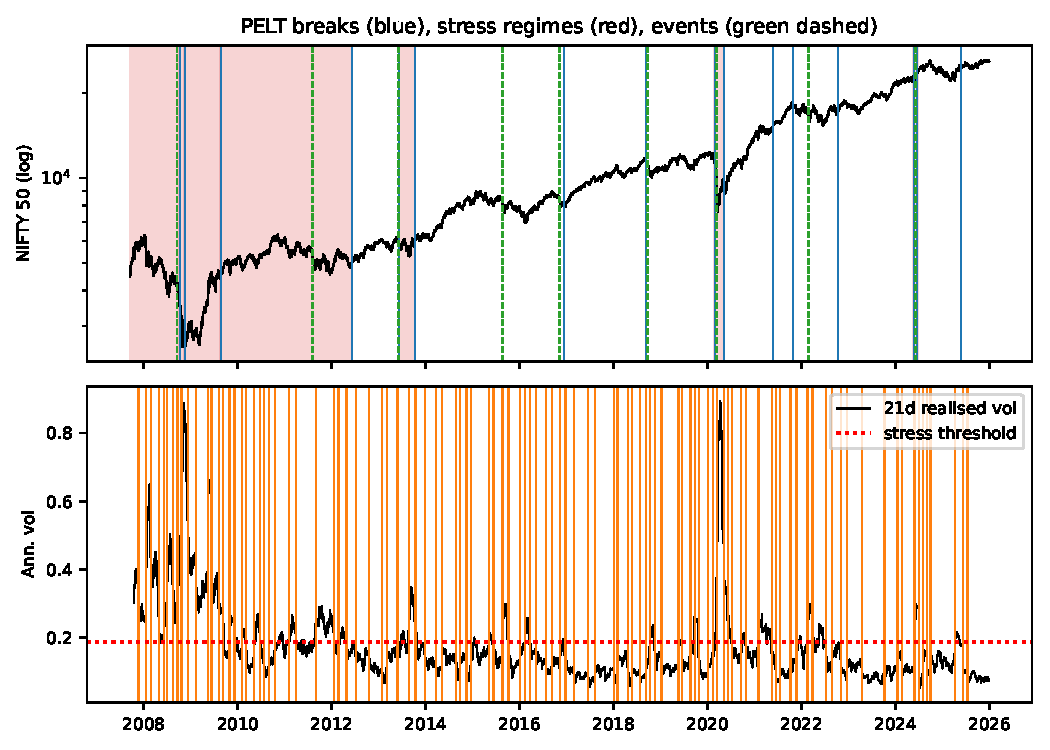
\includegraphics[width=0.85\textwidth]{../figures/cpd_overview.pdf}
\caption{Top: NIFTY~50 with PELT breakpoints on returns (blue), stress segments (red) and event dates (green dashed). Bottom: 21-day realised volatility with the stress threshold and breakpoints from the log-volatility PELT (orange).}\label{fig:cpd}
\end{figure*}

\section{Results}
\subsection{Detected change points and event validation}
PELT on returns finds 16 breaks (Fig.~\ref{fig:cpd}), including 2008-10-06, 2013-06-11, 2016-12-09, 2018-09-10, 2020-02-27, 2022-10-12 and 2024-05-23/06-21; 29\% of days are labelled stress. PELT on log-volatility is far more granular (105 breaks at $\beta{=}2$, 33 at $\beta{=}20$, 14 at $\beta{=}40$) because the smoothed series moves continuously.
Table~\ref{tab:val} shows that PELT on returns matches 56\% of events at $\pm$20 days and 67\% at $\pm$40, against 14\% and 25\% for 16 random breaks. Its precision (38\%) is limited because several breaks mark shifts we did not list. Log-volatility PELT at 105 breaks reaches 100\% recall, but 105 random breaks already reach 62\%, so this mostly reflects density; at a count-matched 14 breaks it attains 33\% recall and 21\% precision. The HMM reaches 67\% recall with 43 switches. Full-sample CPD and HMM regime labels agree on 84.1\% of days (HMM labels 19\% of days stress, CPD 29\%). These results show that PELT localises shifts near documented events better than chance; they do not show timely detection.

\begin{table}[t]\centering\caption{Event validation at $\pm$20 trading days (and recall at $\pm$40).}\label{tab:val}
\footnotesize\begin{tabular}{@{}lrrrr@{}}\toprule
Method & Breaks & Prec. & Rec. & Rec.$_{40}$\\\midrule
PELT, Gaussian, returns & 16 & .375 & .556 & .667\\
PELT, L2, log-vol ($\beta{=}2$) & 105 & .114 & 1.00 & 1.00\\
PELT, L2, log-vol ($\beta{=}40$) & 14 & .214 & .333 & .444\\
Binary seg., L2, log-vol & 102 & .118 & 1.00 & 1.00\\
HMM (2 states) & 43 & .233 & .667 & .667\\
Random ($k{=}16$) & 16 & .082 & .136 & .250\\
Random ($k{=}105$) & 105 & .083 & .619 & .851\\\bottomrule
\end{tabular}\end{table}

\subsection{Forecasting next-21-day volatility}
Table~\ref{tab:fv} and Fig.~\ref{fig:fc} (left) give the out-of-sample results ($T=637$ forecasts, 2013-09-23 to 2025-12-01). The baseline F0 explains 33.3\% of the squared error of the expanding mean; the naive ``last 21-day vol'' forecast is significantly worse than F0 ($p=0.005$), so the trailing/EWMA mix is a meaningful baseline.
\emph{Regime features do not help.} Adding CPD features (F1) changes $R^2_{\mathrm{F0}}$ by $-2.2\%$ ($p=0.62$) and adding the HMM probability (F2) by $-1.2\%$ ($p=0.28$): neither is distinguishable from F0, and both point estimates are negative. Regime features alone (CPD+HMM-only) are far worse than F0 ($-41.5\%$, $p=0.002$).
\emph{VIX does help.} F3 improves on F0 by $+16.6\%$ ($p=0.006$), and VIX alone is the best model ($R^2_{\mathrm{mean}}=0.452$, $+17.8\%$ vs.\ F0, $p=0.042$). Adding the regime features on top of VIX (F4) gives $+14.0\%$ against F0, below F3's $+16.6\%$ (not tested formally): the regime features add noise, not signal, once VIX is present.

\begin{table}[t]\centering\caption{Task V, out-of-sample ($T{=}637$). Target: log 21-day realised vol. DM $p$-values are against F0 (two-sided, HAC $L{=}20$).}\label{tab:fv}
\footnotesize\begin{tabular}{@{}lrrrr@{}}\toprule
Model & RMSE & $R^2_{\mathrm{mean}}$ & $R^2_{\mathrm{F0}}$ & DM $p$\\\midrule
Expanding mean & .4114 & 0 & & \\
Naive (last 21d vol) & .3758 & .166 & $-$.251 & .005\\
F0 trailing+EWMA & .3360 & .333 & 0 & \\
F1 +CPD & .3397 & .318 & $-$.022 & .618\\
F2 +HMM & .3379 & .326 & $-$.012 & .275\\
F3 +VIX & .3067 & .444 & +.166 & .006\\
F4 +VIX+CPD+HMM & .3116 & .427 & +.140 & .043\\
VIX only & .3045 & .452 & +.178 & .042\\
CPD+HMM only & .3996 & .057 & $-$.415 & .002\\\bottomrule
\end{tabular}\end{table}

\begin{figure*}[t]\centering
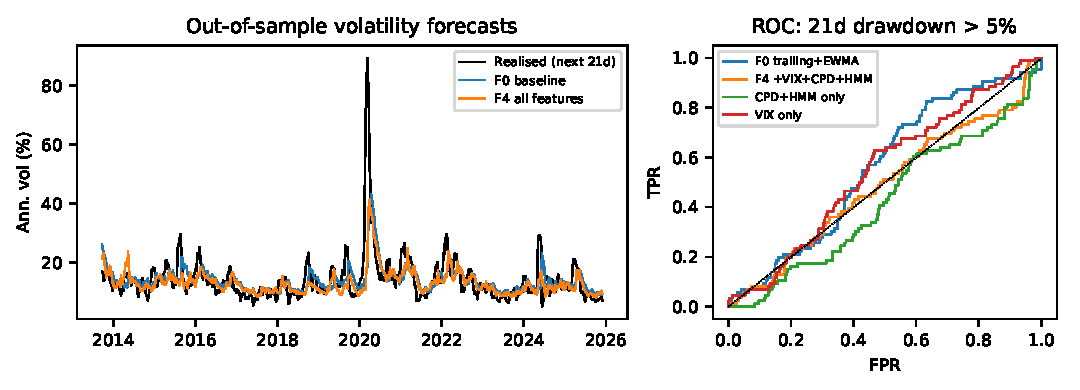
\includegraphics[width=0.85\textwidth]{../figures/forecast.pdf}
\caption{Left: realised next-21-day volatility and out-of-sample forecasts from F0 and F4. Right: ROC curves for the 5\% drawdown flag.}\label{fig:fc}
\end{figure*}

\subsection{Forecasting the 5\% drawdown flag}
Table~\ref{tab:fd} shows that no model discriminates the drawdown flag: AUCs lie between 0.43 and 0.56, and the 95\% block-bootstrap interval for each model's AUC gain over F0 contains zero (e.g.\ F1: $[-0.166,\,0.039]$; F4: $[-0.182,\,0.025]$). Brier scores differ from the base-rate benchmark (0.1228) by under 0.003 in either direction. The CPD+HMM-only model has AUC $0.425<0.5$, i.e.\ worse than chance out of sample. With only 86 positives clustered in a handful of episodes, the effective sample size is small, so these results are also low-powered; the safe conclusion is ``no detectable skill'', not ``proven skill-free''.

\begin{table}[t]\centering\caption{Task D, out-of-sample. $\Delta$AUC is the gain over F0 (95\% block-bootstrap CI).}\label{tab:fd}
\footnotesize\begin{tabular}{@{}lrrrr@{}}\toprule
Model & AUC & Brier & LogLoss & $\Delta$AUC CI\\\midrule
F0 trailing+EWMA & .558 & .1219 & .4085 & \\
F1 +CPD & .502 & .1206 & .4171 & [$-$.166,.039]\\
F2 +HMM & .531 & .1223 & .4129 & [$-$.079,.010]\\
F3 +VIX & .560 & .1230 & .4114 & [$-$.025,.032]\\
F4 all & .486 & .1228 & .4251 & [$-$.182,.025]\\
VIX only & .547 & .1203 & .4059 & [$-$.095,.058]\\
CPD+HMM only & .425 & .1267 & .4320 & [$-$.309,.022]\\
Base rate only & .500 & .1228 & .4148 & \\\bottomrule
\end{tabular}\end{table}

\subsection{What the regime signals do tell us}
Table~\ref{tab:cond} shows that, descriptively, the regime signals \emph{do} separate calm from volatile futures: next-21-day volatility averages 18.2\% when the CPD flag is on versus 13.0\% when off, and 17.3\% versus 13.1\% for the HMM; the HMM stress state also precedes a 5\% drawdown 20.0\% of the time versus 11.3\%. This is volatility persistence at work. But this information is already contained in trailing and EWMA volatility, which is why the regime features add nothing in the regressions above. Standardised coefficients of the all-feature model fitted on all 791 samples (descriptive, in-sample) point the same way: India VIX dominates the volatility ridge model (0.238, against 0.055 for trailing vol and at most 0.041 in absolute value for each CPD and HMM term).

\begin{table}[t]\centering\caption{Conditional out-of-sample outcomes (no model fitted; overlapping windows, not significance-tested).}\label{tab:cond}
\footnotesize\begin{tabular}{@{}lrrr@{}}\toprule
Condition & $n$ & Mean vol & Freq. dd$>$5\%\\\midrule
CPD flag = 1 & 144 & .182 & .146\\
CPD flag = 0 & 493 & .130 & .132\\
HMM $P$(stress) $>$ .5 & 160 & .173 & .200\\
HMM $P$(stress) $\le$ .5 & 477 & .131 & .113\\
India VIX $>$ 25 & 33 & .278 & .152\\
India VIX $\le$ 25 & 604 & .134 & .134\\\bottomrule
\end{tabular}\end{table}

\subsection{Allocation backtest}
Table~\ref{tab:bt} and Fig.~\ref{fig:bt} (3~Jan.\ 2011--30~Dec.\ 2025) show that every regime rule reduced maximum drawdown by about 11--12 points relative to buy-and-hold. Only the HMM rule also improved return and Sharpe (0.59 vs.\ 0.46); the CPD rule lost return (7.6\% vs.\ 10.4\%) and the VIX rule did worst. The static 60/40 NIFTY/gold mix beat every regime strategy; since gold rallied strongly over the period, much of the benefit of ``moving to gold'' is a gold effect rather than a timing effect. This is consistent with the forecasting results: if regime signals add no incremental information on future risk, timing on them should not produce reliable gains.

\begin{table}[t]\centering\caption{Walk-forward allocation, Jan.\ 2011--Dec.\ 2025, 10~bp costs.}\label{tab:bt}
\footnotesize\begin{tabular}{@{}lrrrrr@{}}\toprule
Strategy & CAGR\% & Vol\% & Sharpe & MaxDD\% & Sw.\\\midrule
Buy \& hold NIFTY & 10.39 & 16.5 & 0.46 & $-$38.4 & 0\\
Static 60/40 NIFTY/Gold & 12.04 & 12.0 & 0.71 & $-$25.8 & 0\\
CPD regime (walk-fwd) & 7.58 & 15.0 & 0.32 & $-$26.1 & 18\\
HMM regime (walk-fwd) & 11.19 & 13.4 & 0.59 & $-$26.1 & 36\\
VIX$>$25 rule & 5.74 & 13.9 & 0.21 & $-$27.1 & 84\\\bottomrule
\end{tabular}\end{table}
\begin{figure}[t]\centering
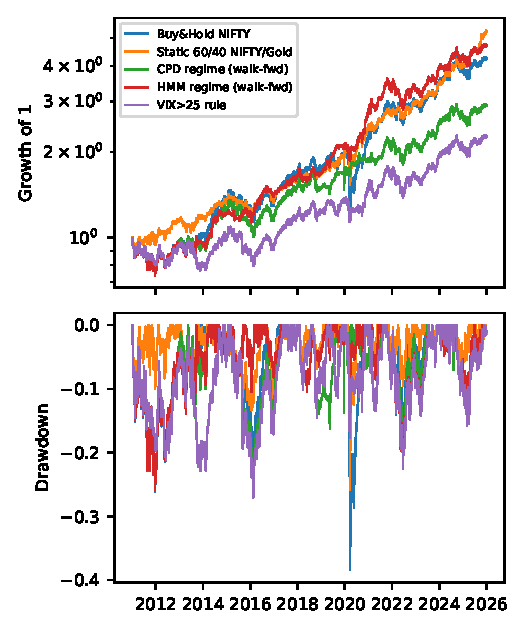
\includegraphics[width=0.85\columnwidth]{../figures/backtest.pdf}
\caption{Growth of one rupee (log scale) and drawdowns.}\label{fig:bt}
\end{figure}

\section{Discussion and Limitations}
\emph{Multiple comparisons.} Seven feature sets and two tasks were compared without correction for multiple testing; the single positive result that survives (VIX) is also the most economically plausible. \emph{Overlap.} Weekly samples with 21-day targets overlap by about 80\%; the DM test and block bootstrap address serial dependence, but the effective number of independent forecasts is far below 637. \emph{Few episodes.} The drawdown task rests on 86 positives from a handful of episodes. \emph{Fixed hyperparameters.} We chose not to tune $\alpha$, $C$, $\beta$ or the 1.3 stress multiple to avoid selection bias; a tuned or non-linear model (e.g.\ gradient boosting) might extract more, and this is untested. \emph{Penalty sensitivity.} Breakpoint count, and hence event precision and recall, depend strongly on $\beta$. \emph{Event dates.} The nine dates were chosen by us, are approximate, and need source verification. \emph{Detection lag.} We did not measure the real-time delay from an event to the first stress signal, so the idea that late signals explain the CPD allocation drag is plausible but untested. \emph{Single path.} One 15-year history, no confidence intervals on the backtest. \emph{Data.} Yahoo Finance data and ETF proxies; taxes and slippage beyond 10~bp are ignored.

\section{Conclusion}
Offline CPD localises stress-related shifts in the NIFTY~50 well above chance, and complements the HMM by returning fewer, penalty-controlled regimes. But these regimes describe volatility rather than predict it: in a strictly out-of-sample weekly walk-forward test with embargoed training sets, CPD and HMM features did not improve forecasts of next-month volatility over trailing and EWMA volatility, did not help predict a 5\% drawdown, and were dominated by India VIX. In allocation they reduced drawdown but did not reliably raise risk-adjusted returns. We therefore find no evidence of an alpha signal in regime detection itself. Future work: online CPD for measured detection delay, leading indicators (flows, credit spreads, option skew), tuned and non-linear models, and formal multiple-testing control.

\begin{thebibliography}{9}\small
\bibitem{killick} R. Killick, P. Fearnhead, and I. A. Eckley, ``Optimal detection of changepoints with a linear computational cost,'' \emph{J. Amer. Statist. Assoc.}, vol. 107, no. 500, pp. 1590--1598, 2012.
\bibitem{truong} C. Truong, L. Oudre, and N. Vayatis, ``Selective review of offline change point detection methods,'' \emph{Signal Processing}, vol. 167, 2020.
\bibitem{angtim} A. Ang and A. Timmermann, ``Regime changes and financial markets,'' \emph{Annu. Rev. Financ. Econ.}, vol. 4, pp. 313--337, 2012.
\bibitem{hamilton} J. D. Hamilton, ``A new approach to the economic analysis of nonstationary time series and the business cycle,'' \emph{Econometrica}, vol. 57, no. 2, pp. 357--384, 1989.
\bibitem{adams} R. P. Adams and D. J. C. MacKay, ``Bayesian online changepoint detection,'' arXiv:0710.3742, 2007.
\bibitem{dm} F. X. Diebold and R. S. Mariano, ``Comparing predictive accuracy,'' \emph{J. Bus. Econ. Statist.}, vol. 13, no. 3, pp. 253--263, 1995.
\bibitem{nw} W. K. Newey and K. D. West, ``A simple, positive semi-definite, heteroskedasticity and autocorrelation consistent covariance matrix,'' \emph{Econometrica}, vol. 55, no. 3, pp. 703--708, 1987.
\bibitem{kunsch} H. R. K\"unsch, ``The jackknife and the bootstrap for general stationary observations,'' \emph{Ann. Statist.}, vol. 17, no. 3, pp. 1217--1241, 1989.
\bibitem{rm} J. P. Morgan/Reuters, \emph{RiskMetrics---Technical Document}, 4th ed., New York, 1996.
\end{thebibliography}
\end{document}
